\documentclass[12pt,a4paper,bibliography=totocnumbered,listof=totocnumbered]{scrartcl}

\usepackage[ngerman]{babel}
\usepackage[utf8]{inputenc}
\usepackage{amsmath}
\usepackage{amsfonts}
\usepackage{amssymb}
\usepackage{graphicx}
\usepackage{fancyhdr}
\usepackage{tabularx}
\usepackage{geometry}
\usepackage{setspace}
\usepackage[right]{eurosym}
\usepackage[printonlyused]{acronym}
\usepackage{subfig}
\usepackage{floatflt}
\usepackage[usenames,dvipsnames]{color}
\usepackage{colortbl}
\usepackage{paralist}
\usepackage{array}
\usepackage{titlesec}
\usepackage{parskip}
\usepackage{acronym}
\usepackage[modulo]{lineno}
\pagewiselinenumbers
\usepackage{footmisc}
\usepackage[right]{eurosym}
\usepackage[subfigure,titles]{tocloft}
\usepackage[pdfpagelabels=true]{hyperref}
\usepackage{comment}
\usepackage{csquotes}

\usepackage{listings}
\lstset{basicstyle=\footnotesize, captionpos=b, breaklines=true, showstringspaces=false, tabsize=2, frame=lines, numbers=left, numberstyle=\tiny, xleftmargin=2em, framexleftmargin=2em}
\def\l@lstlisting#1#2{\@dottedtocline{1}{0em}{1em}{\hspace{1,5em} Lst. #1}{#2}}
\makeatother
\makeatletter

\geometry{a4paper, top=27mm, left=30mm, right=20mm, bottom=35mm, headsep=10mm, footskip=12mm}

\hypersetup{unicode=false, pdftoolbar=true, pdfmenubar=true, pdffitwindow=false, pdfstartview={FitH},
	pdftitle={Bachelorarbeit},
	pdfauthor={Fabian Wilms},
	pdfsubject={Bachelorarbeit},
	pdfcreator={\LaTeX\ with package \flqq hyperref\frqq},
	pdfproducer={pdfTeX \the\pdftexversion.\pdftexrevision},
	pdfkeywords={Bachelorarbeit},
	pdfnewwindow=true,
	colorlinks=true,linkcolor=black,citecolor=black,filecolor=magenta,urlcolor=black}
\pdfinfo{/CreationDate (D:20110620133321)}
% ----------------------------------------------------------------------------------------------------------
% Eigene Befehle
% ----------------------------------------------------------------------------------------------------------

% Image Command
% #1 IMAGE File
% #2 Caption
\newcommand{\image}[2]{
	\vspace{1em}
	\begin{minipage}{\linewidth}
		\centering
		\includegraphics[width=0.9\linewidth]{#1}
		\captionof{figure}{#2}
		\label{fig:#1}
	\end{minipage}
}

% Quote Command
% #1 Quote Text
\newcommand{\myquote}[1]{
	\begin{quote}
		\begin{itshape}
			\enquote{#1}
		\end{itshape}
	\end{quote}
}
%-------------

\begin{document}

\titlespacing{\section}{0pt}{12pt plus 4pt minus 2pt}{-6pt plus 2pt minus 2pt}

% Kopf- und Fusszeile
\renewcommand{\sectionmark}[1]{\markright{#1}}
\renewcommand{\leftmark}{\rightmark}
\pagestyle{fancy}
\lhead{}
\chead{}
\rhead{\thesection\space\contentsname}
\lfoot{Generative Testerstellung für Microservice-Architekturen}
\cfoot{}
\rfoot{Seite \thepage}
\renewcommand{\headrulewidth}{0.4pt}
\renewcommand{\footrulewidth}{0.4pt}

% Vorspann
\renewcommand{\thesection}{\Roman{section}}
\renewcommand{\theHsection}{\Roman{section}}
\pagenumbering{Roman}

% ----------------------------------------------------------------------------------------------------------
% Titelseite
% ----------------------------------------------------------------------------------------------------------
\thispagestyle{empty}
\begin{center}
	
\includegraphics[scale=0.25]{images/Hochschule_Muenchen_Logo.png}\\
	\vspace*{2cm}
	\Large
	\textbf{Fakultät für Informatik und Mathematik 07}\\
	\vspace*{2cm}
	\Huge
	\textbf{Bacheloararbeit}\\
	\vspace*{0.5cm}
	\large
	über das Thema\\
	\vspace*{1cm}
	\textbf{Generative Testerstellung für Microservice-Architekturenit}\\
	\vspace*{2cm}
	
	\vfill
	\normalsize
	\newcolumntype{x}[1]{>{\raggedleft\arraybackslash\hspace{0pt}}p{#1}}
	\begin{tabular}{x{6cm}p{7.5cm}}
		\rule{0mm}{5ex}\textbf{Autor:} & Fabian Wilms\newline holtkoet@hm.edu \\ 
		\rule{0mm}{5ex}\textbf{Prüfer:} & Prof. Dr. Ulrike Hammerschall \\ 
		\rule{0mm}{5ex}\textbf{Abgabedatum:} & xx.xx.2017 \\ 
	\end{tabular} 
\end{center}
\pagebreak

% ----------------------------------------------------------------------------------------------------------
% Abstract
% ----------------------------------------------------------------------------------------------------------
\setcounter{page}{1}
\onehalfspacing
\titlespacing{\section}{0pt}{12pt plus 4pt minus 2pt}{2pt plus 2pt minus 2pt}
\rhead{KURZFASSUNG}
\section{Kurzfassung}

kurzfassung

\vspace{-1,2em}
\titlespacing{\section}{0pt}{12pt plus 4pt minus 2pt}{-6pt plus 2pt minus 2pt}
\section*{Abstract}

Das ganze auf Englisch.

\pagebreak

% ----------------------------------------------------------------------------------------------------------
% Verzeichnisse
% ----------------------------------------------------------------------------------------------------------
% TODO Typ vor Nummer
\renewcommand{\cfttabpresnum}{Tab. }
\renewcommand{\cftfigpresnum}{Abb. }
\settowidth{\cfttabnumwidth}{Abb. 10\quad}
\settowidth{\cftfignumwidth}{Abb. 10\quad}

\titlespacing{\section}{0pt}{12pt plus 4pt minus 2pt}{2pt plus 2pt minus 2pt}
\singlespacing
\rhead{INHALTSVERZEICHNIS}
\renewcommand{\contentsname}{II Inhaltsverzeichnis}
\phantomsection
\addcontentsline{toc}{section}{\texorpdfstring{II \hspace{0.35em}Inhaltsverzeichnis}{Inhaltsverzeichnis}}
\addtocounter{section}{1}
\tableofcontents
%\pagebreak
\rhead{VERZEICHNISSE}
\listoffigures
%\pagebreak
\listoftables
%\pagebreak
\renewcommand{\lstlistlistingname}{Listing-Verzeichnis}
{\labelsep2cm\lstlistoflistings}
%\pagebreak

% ----------------------------------------------------------------------------------------------------------
% Abkürzungen
% ----------------------------------------------------------------------------------------------------------
\section{Abkürzungsverzeichnis}
\begin{acronym}[HATEOAS] % längste Abkürzung steht in eckigen Klammern
	\acro{DDD}{Domain-Driven Design}
	\acro{LHM}{Landeshauptstadt München}
	\acro{LDAP}{Lightweight Directory Access Protocol}
	\acro{HATEOAS}{Hypermedia as the engine of application state}
	\acro{RPC}{Remote Procedure Call}
	\acro{REST}{Representational State Transfer}
	\acro{API}{Application Programming Interface}
	\acro{ORM}{Object-Relational Mapping}
\end{acronym}
\newpage

% ----------------------------------------------------------------------------------------------------------
% Inhalt
% ----------------------------------------------------------------------------------------------------------
% Abstände Überschrift
\titlespacing{\section}{0pt}{12pt plus 4pt minus 2pt}{-6pt plus 2pt minus 2pt}
\titlespacing{\subsection}{0pt}{12pt plus 4pt minus 2pt}{-6pt plus 2pt minus 2pt}
\titlespacing{\subsubsection}{0pt}{12pt plus 4pt minus 2pt}{-6pt plus 2pt minus 2pt}

% Kopfzeile
\renewcommand{\sectionmark}[1]{\markright{#1}}
\renewcommand{\subsectionmark}[1]{}
\renewcommand{\subsubsectionmark}[1]{}
\lhead{Kapitel \thesection}
\rhead{\rightmark}

\onehalfspacing
\renewcommand{\thesection}{\arabic{section}}
\renewcommand{\theHsection}{\arabic{section}}
\setcounter{section}{0}
\pagenumbering{arabic}
\setcounter{page}{1}
\setcounter{secnumdepth}{6}

% ----------------------------------------------------------------------------------------------------------
% Einführung und Motivation
% ----------------------------------------------------------------------------------------------------------
\section{Einführung und Motivation}

IT nimmt sowohl im privaten als auch geschäftlichen Alltag eine immer größere Rolle ein. Die Übernahme von Bereichen, die ehemals als nicht durch Computer austauschbar erachtet wurden, schreitet immer weiter fort. Doch dadurch steigen nicht nur bestehende Anforderungen an Software, sondern es entstehen auch neue Kriterien an die Qualität. Sobald Türklingeln, Alarmanlagen und Schließanlagen \textit{smart} werden, ist die Fehlertoleranz gleich null. Ganz abgesehen davon steigt auch die Komplexität von modernen Software-Systemen immens an.

Mit steigender Komplexität und höherer Nachfrage am Markt, sowie engen Zeitplänen für Projekte wird leider häufig aus Zeit- und Kostengründen auf Qualität nur geringfügig Rücksicht genommen. Zunächst verursacht eine gute Software-Qualität nämlich Mehrkosten. Personelle wie zeitliche. Dies zeigt das Magische Dreieck, oder im englischen das Project Management Triangle.

\image{images/img_magisches_dreieck.pdf}{Magisches Dreieck des Projektmanagements\cite{hagen}}

Dieses besagt, dass die Qualität eines Projekts durch die drei Faktoren der Leistung, Kosten und Zeit beeinflusst wird. Diese Faktoren müssen vom Management eines Projekts möglichst ausbalanciert gehalten werden. Beispiel anhand des Hausbaus: Vom Bauherren ist ein fester Termin für die Fertigstellung des Hauses angedacht (Faktor Zeit), doch lässt der aktuelle Baufortschritt eine Fertigstellung zum festgelegten Termin nicht mehr zu. Die Lösung wäre, mehr Arbeiter einzustellen und somit den Fortschritt zu beschleunigen. Somit werden zum Ausgleich die Kosten erhöht.

Ein Bericht der Kölner Beratungsfirma SQS zeigt anhand von gesammelten Zahlen aus Beratungsaufträgen welche immensen Kosten durch unentdeckte Fehler entstehen \cite{sqsdefect}. Hier wird besonders deutlich wie viel es für ein Projekt bedeutet, frühzeitige Qualitätssicherung durchzusetzen. Und dazu zählt auch das Testen von Software.

\image{images/img_sqs-defect-correction.PNG}{SQS Report Costs of Defect Correction \cite{sqsdefect}}

Umso früher Fehler entdeckt und bemerkt werden, umso weniger kostet es auch diese zu beheben. Wenn bereits vor dem Start der Implementierungsphase auf eine hohe Testabdeckung, beispielsweise durch den Einsatz von test-driven development, wert gelegt wird, können, je auftretendem Fehler, um die 7800\euro\ \cite{sqsdefect} eingespart werden. Mit diesen Zahlen sind die Mehrkosten, die für ein solches vorgehen entstehen um ein vielfaches leichter zu rechtfertigen.

Somit sorgt das Bug-Fixing in Produktivsystemen, also das Beheben sogenannter \textit{field defects}, für einen der größten Kostenfaktoren. Wurde in den ersten Phasen eines Projekts nicht viel, oder kein Wert auf eine ausreichende Test-Abdeckung gelegt schaffen es viele Fehler in die Produktivsysteme der Hersteller. Doch werden diese Fehler erst im laufenden Betrieb beim Kunden festgestellt, ist es bereits zu spät. Robert N. Charette kritisiert eben dies in seinem Artikel \textit{Why Software Fails}\cite{charette}.

\myquote{If the software coders don't catch their omission until final system testing--or worse, until after the system has been rolled out--the costs incurred to correct the error will likely be many times greater than if they'd caught the mistake while they were still working on the initial [...] process.}

Die Lösung sollte also sein, viel Zeit und Geld in gute Softwarequalität zu investieren. Jedoch stehen, wie bereits am Anfang der Einleitung erwähnt, Projektleiter und ihre Mitarbeiter unter hohem zeitlichen Druck vom Kunden oder durch andere beteiligte festgelegte Termine einzuhalten. Und gute Tests kosten neben Geld auch Zeit. Es entsteht in dieser Zeit aber kein Fortschritt an der Funktionalität der Software.

Bei it@M, dem IT-Dienstleister der Landeshauptstadt München, ist eine hohe Testabdeckung daher Teil der Definition of Done [citation needed] von Softwareprojekten. Im Kommunalen Umfeld sind die zeitlichen Restriktionen noch einmal stärker zu gewichten als in der freien Wirtschaft. Viele Projekte werden aufgrund von anstehenden Gesetzesänderungen ins Leben gerufen und müssen mit Inkrafttreten der neuen Regelungen in Produktion gehen. it@M ist somit ständig auf der Suche nach Lösungen, die den Entwicklungs- und Testprozess beschleunigen, um die geringe Zeit möglichst effizient nutzen zu können.

Eine dieser Lösungen wurde im letzten Jahr von Martin Kurz im Rahmen seiner Masterarbeit \cite{mkthesis} geplant und entwickelt. Die Model-driven Software Development Lösung Barrakuda \footnote{Github Repository von Barrakuda (https://github.com/xdoo/mdsd)}. Diese bietet den Entwicklern von it@M die Möglichkeit anhand von einer vorgegebenen Domänen-spezifischen Sprache Microservice-Architekturen zu modellieren und diese zu generieren.

Im Rahmen dieser Arbeit soll eine Erweiterung von Barrakuda geplant und entwickelt werden. Diese Weiterentwicklung soll einen Großteil verschiedener Testmethoden für diese Architektur generieren und die benötigte Entwicklungszeit für eine hohe Testabdeckung möglichst stark reduzieren.

Zunächst werden die Microservice Architektur (Kapitel~\ref{ch:ms-arch}) und der Monolithischen Architekturstil (Kapitel~\ref{ch:mon-arch}) beschrieben und bezüglich ihrer Vor- (Kapitel~\ref{ch:ms-mon-pro}) und Nachteile (Kapitel~\ref{ch:ms-mon-cons}) verglichen. Anschließend wird ein praktisches Beispiel anhand der von it@M Vorgegebene Microservice-Architektur gezeigt und die zu testenden Komponenten identifiziert.

Schließlich werden bekannte Methoden zum Testen von Software analysiert (Kapitel~\ref{ch:soft-test}) und es werden alternative Methoden, die besonders im Bereich der Microservices anzutreffen sind, ebenfalls untersucht (Kapitel~\ref{ch:ms-test}). Diese werden dann in Hinblick der Umsetzungsmöglichkeit im generativen Ansatz geprüft (Kapitel~\ref{ch:ms-gen-test})  und es werden Frameworks die zur Implementierung genutzt werden sollen definiert(Kapitel~\ref{ch:ms-test-frw}) .

Schließlich sollen Anforderungen, die an die zu generierenden Tests gestellt werden (Kapitel~\ref{ch:anforderungen-tests}), festgehalten werden. Diese finden dann im letzten Abschnitt, der Implementierung, Beachtung (Kapitel~\ref{ch:implementierung}).

% ----------------------------------------------------------------------------------------------------------
% Architektur-Generierung für Software-Projekte
% ----------------------------------------------------------------------------------------------------------
\section{Architekturvergleich Microservice und Monolith}

Architekturen gibt es in der Welt der Softwareentwicklung viele. Eine der momentan bekanntesten Neuerungen an den Whiteboards der IT-Architekten ist die "Microservice" Architektur. Viele kleine Services die im Konglomerat für ein gemeinsames Ziel zusammenarbeiten. Vorbei sein soll die Zeit der Monolithischen Softwaresysteme, bei denen die Gesamtlogik in einer einzigen Anwendung gekapselt ist.

\image{images/img_monolith-vs-ms.pdf}{Logische Unterscheidung zwischen Monolithischer und Microservice Architektur}

Sam Newman stellt in seinem Buch \textit{Building Microservices}\cite{buildingms} einige Vorteile dar, die Microservices gegenüber Monolithischen Architekturen bieten. Doch um diese Vorteile besser zu verstehen muss man zunächst die Unterschiede der zwei Architekturstile im Detail betrachten.

\subsection{Microservice Architektur}\label{ch:ms-arch}

Um die Vorteile dieser Architektur in einem System effektiv zu nutzen gibt es bereits in der Planung einiges zu beachten.

Dazu zählt, dass es zwei Dinge gibt, die einen guten Microservice ausmachen. Lose Kopplung und Starker Zusammenhalt \cite[S.62]{buildingms}.

Lose Kopplung bedeutet, dass Änderungen an einem Service keine Änderungen an einem anderen Service nach sich ziehen. Ist dies nicht gegeben, ist einer der Hauptvorteile von dieser Art Architektur nicht mehr vorhanden.
Ein lose gekoppelter Service weiß von seinem Kommunikationspartner nur so wenig wie möglich.\cite[S.63]{buildingms}

Starker Zusammenhalt soll dafür sorgen, dass bestimmte Funktionalitäten an einem Ort vorhanden sind, sodass diese leicht geändert werden können und nicht mehrere Komponenten angepasst werden müssen.\cite[S.64]{buildingms}

Zum Planen einer Software mit Mircoservice Architektur ist es sinnvoll, sich zunächst über Kontextgrenzen (\textit{bounded context}) Gedanken zu machen. Kontextgrenzen sind eine Definition aus dem Buch \textit{Domain Driven Design} von Eric Evans \cite{dddesign}.

Sie lassen sich gut am Beispiel eines Online-Shops zeigen. Wenn ein Online-Shop geplant wird ist einer der zentralen Bestandteile die Lagerverwaltung. Die Daten der Lagerverwaltung werden herangezogen um dem potentiellen Kunden des Shops anzuzeigen welche und wie viele Produkte verfügbar sind. Doch möchte ein Kunde nun ein Produkt bestellen hat dies nichts mehr mit einer Lagerverwaltung, sondern mit einem Bestellsystem zu tun. Man verlässt also den ursprünglichen Kontext der Lagerverwaltung. Somit entsteht in der Planung eine neue Kontextgrenze: Die des Bestellsystems. Es verwaltet Bestellungen von Kunden. Doch woher kommen die Kundendaten? Kundendaten haben zwar einen Verwendungszweck im Bestellsystem, doch die Verwaltung der Daten hat mit der eigentlichen Kompetenz dieses Systems nichts mehr zu tun. Somit wird eine weitere Kontextgrenze erstellt, nämlich die der Kundenverwaltung.

Eine Kontextgrenze soll also eine logische Grenze darstellen, welche eventuell über eine oder mehrere Schnittstellen verfügt, die festlegen, welche Informationen mit anderen Kontexten geteilt werden.\cite[S.65]{buildingms}. Damit einher geht die Unterscheidung zwischen geteilten und versteckten Modellen. Versteckte Modelle werden innerhalb einer Kontextgrenze benötigt, sind aber für andere Kontexte uninteressant. Geteilte Modelle hingegen werden über die Grenzen hinweg freigegeben. Sind solche Kontextgrenzen für eine Software modelliert, lassen sich aus diesen sehr leicht Microservices ableiten, da bereits einige Grundvoraussetzungen getroffen sind: Lose Kopplung und Starker Zusammenhalt.\cite[S.68]{buildingms}

\myquote{[I]f our service boundaries align to the bounded contexts in our domain, and our microservices
	represent those bounded contexts, we are off to an excellent start in ensuring that our microservices
	are loosely coupled and strongly cohesive.\cite{buildingms}}

\subsubsection{Kommunikation zwischen Services}

Als weiterer Schritt muss eine Kommunikationsart zwischen Services und zur Außenwelt definiert werden.

\paragraph{Geteilte Datenbanken} sind eine Möglichkeit zur Servicekommunikation \cite[S.85]{buildingms}. Die Idee hinter dieser Art der Kommunikation ist besonders trivial. Mehrere Services, die miteinander Daten austauschen wollen, nutzen eine gemeinsame Datenbank. Jeder Service hat somit jederzeit Zugriff zu allen Daten der anderen Nutzer dieser geteilten Datenbank und es findet somit keine \textit{echte} Kommunikation statt, sondern nur Zugriffe auf geteilten Speicher.\cite{shareddb}
Dies birgt natürlich viele Probleme. Jede noch so kleine Änderung an der "Logik" dieser Datenbank, oder an der internen Struktur der Daten muss mit viel Bedacht durchgeführt werden, da jede abhängige Komponente sonst nicht mehr funktionieren könnte.

Des Weiteren ist die technologische Einschränkung ein großer Nachteil. Wenn es auch in den ersten Schritten der Planung und Entwicklung Sinnvoll erscheint eine relationale Datenbank zu verwenden, können spätere Geschäftsentscheidungen oder neu auftretende Probleme den Einsatz einer Graphdatenbank sinnvoller machen. Bei einer geteilten Datenbank eine solche Änderung durchzuführen ist sehr schwierig\cite[S.85]{buildingms}.

\paragraph{\acf{RPC}s}\label{rpcpara} sind eine weitere bekannte Kommunikationsmöglichkeit. Die Übersetzung ins deutsche erklärt schon einen Großteil der Idee hinter \ac{RPC}s: "Aufruf einer fernen Prozedur". \ac{RPC}s sind eine weitere Möglichkeit eine Client-Server-Modell umzusetzen. Die erste Idee dazu kam im Jahre 1976 von James White in seinem RFC \#707 \enquote{A High-Level Framework for Network-Based Resource Sharing}\cite{white707}. Ein \ac{RPC} funktioniert, indem der Client einer Anwendung eine Anfrage an einen Server sendet. In dieser Anfrage ist der Name oder die ID einer Methode, sowie die zugehörigen Parameter enthalten. Der empfangende Server führt die gewünschte Methode bei sich aus und liefert dem Client als Antwort den Rückgabewert der Methode.
Ein Vorteil von RPC ist, dass es sehr einfach und schnell möglich ist Methoden der Services für Clients und andere Services Verfügbar zu machen. Über die Kommunikation muss man sich nahezu keine Gedanken machen\cite[S.91]{buildingms}.

Doch die Nachteile überwiegen schnell und deutlich. Je nach Implementierung führt die Verwendung von RPC zu einer starken Bindung an eine bestimmte Sprache (bekanntestes Beispiel Java RMI). Auch verstecken RPC-Implementierungen die Komplexität der entfernten Aufrufe. Dies kann zu starken Performance-Problemen führen, wenn Entwickler an Interfaces arbeiten, von denen sie denken es seien lokale Methoden\cite[S.93]{buildingms}.

Die Verwendung von RPC macht die Weiterentwicklung von Systemen nicht einfacher: Ein Beispiel anhand einer Schnittstelle zur Instanziierung eines Kunden. Zusätzlich zur Erstellung eines Kunden mithilfe seines Namen und einer E-Mail Adresse soll es nun eine Möglichkeit geben diesen nur mithilfe seiner Mail-Adresse zu erstellen. Das reine hinzufügen einer neuen Methode in einem Interface löst das Problem in diesem Fall nicht. Im schlimmsten Fall benötigen alle Clients die diesen Service ansprechen die neuen Stubs und müssen allesamt neu Bereitgestellt werden\cite[S.94]{buildingms}. Und das bereits bei einer so kleinen Änderung.

\paragraph{\acf{REST}} ist eine der meistgenutzten Programmierparadigmen für \ac{API}s \cite{duvander}. Entworfen wurde \ac{REST} von Roy Fielding, der die Idee und Spezifikationen in seiner Dissertation \enquote{Architectural Styles and the Design of Network-based Software Architectures} veröffentlichte.\cite{fielding}. Insgesamt besteht Fielding auf 6 Eigenschaften, die erfüllt sein müssen um eine REST-Konforme Anwendung zu schreiben.

Die erste dieser Eigenschaften (\enquote{Client-Server}) verlangt schlichtweg, dass eine Client-Server Architektur vorliegt, bei der ein Server Funktionalität bereitstellt, die der Client nutzen kann.
\enquote{Stateless} ist die zweite Eigenschaft, die von Fielding gefordert wird. Sie besagt, dass alle Informationen, die zum Verständnis einer Nachricht nötig sind auch mitgeliefert werden müssen, da weder der Client, noch der Server, Zustandsinformationen zwischen Anfragen speichern sollen.
Eigenschaft Nummer 3, \enquote{Caching}, fordert die Verwendung von Caching um Netzwerklast zu minimieren.
Das \enquote{Uniform Interface} ist eine der größten Unterschiede von REST zu anderen Netzwerkarchitekturstilen. Diese Eigenschaft ist erneut aufgeteilt in vier Unterpunkte:

\begin{description}  
	\item [Identification of resources] Jede, über eine URI erreichbare Information ist eine Ressource
	\item [Manipulation of resources through representations] Änderungen an Ressourcen erfolgen nur über Repräsentationen von Ressourcen, also zum Beispiel durch Formate wie XML oder JSON. Genauso gut kann eine Ressource aber auch in unterschiedlichen Darstellungsformen vom Server ausgeliefert werden.
	\item [Self-descriptive messages] Die für die Anwendung versendeten Nachrichten sollen selbstbeschreibend sein. Zur Erfüllung dieser Eigenschaft ist es unter anderem nötigt, Standardmethoden zur Manipulierung von Ressourcen zu verwenden.
	\item [\acf{HATEOAS}] ist ein wichtiger Teil der REST-Spezifizierung und beschreibt ein Konzept, nach dem, einfach gesagt, Informationen Links zu anderen Informationen enthalten. 
\end{description}

Die fünfte Eigenschaft verlangt nach \enquote{Layered Systems}, also mehrschichtigen Systemen. Die Idee dahinter ist, dass die Komponenten nur die Komponenten im System kennen mit denen sie in direkter Interaktion stehen. Alles weitere bleibt verborgen.
\enquote{Code-On-Demand} ist die letzte und eine optionale Eigenschaft der Spezifikation. Fielding beschreibt hiermit die Erweiterung von Client-Funktionalität durch den Server. Dieser sendet, wie zum Beispiel mit Javascript der Fall, Code für den Client direkt an den Client,.\cite{fielding}

REST wird, auch wenn die Spezifikation es nicht vorschreibt, in den häufigsten Fällen über HTTP genutzt \cite[S.97]{buildingms}. Dies rührt daher, dass beispielsweise die bekannten HTTP-Methoden POST, GET, PUT usw. es sehr einfach machen die geforderte homogene Verhaltensweise von Methoden auf allen Ressourcen umzusetzen. Auch wird HTTP gerne genutzt, da es bereits eine breite Masse an bestehenden Tools gibt die zur weiteren Qualitätsverbesserung eines Systems genutzt werden können, wie zum Beispiel Proxies und Load Balancer. Doch dies sind alles zunächst nur Vorteile von HTTP.

Die Verwendung von REST bietet viele Möglichkeiten die lose Kopplung zwischen Services zu ermöglichen. Dazu zählt unter anderem \ac{HATEOAS}. Um bei dem Kundenbeispiel aus \ref{rpcpara} zu bleiben: Wird die Information eines Kunden abgerufen, kann das Kundenobjekt zusätzlich zu den Kundendaten ein Feld enthalten welches zur Bestellliste dieses Kund zeigt.

\lstinputlisting{code/customer.json}

Mit der Verwendung von HATEOAS reicht es, wenn alle Clients die Kundendaten und deren Bestellungen verarbeiten wissen, dass Kunden einen Link-Feld mit dem Typ \textit{orders} besitzen. Wenn also später Services unter anderen Adressen erreichbar sind, oder sich interne Datenstrukturen ändern müssen diese Clients nicht neu angepasst werden.

\paragraph{JSON oder XML?} 

Wenn die Entscheidung über die Art und Weise der Datenübertragung gefallen ist muss das Datenformat festgelegt werden. JSON und XML sind dabei die bekanntesten Namen. In den vergangenen Jahren ist dabei die Verwendung von XML im Gegensatz zu JSON in \ac{API}s zurückgegangen\cite{duvander2}. Jedoch bieten beide Vor- wie Nachteile. JSON ist das einfachere Format und auch leichtgewichtiger, während XML einige sinnvolle Features wie z.B. link control (insbesondere für HATEOAS interessant) oder auch das extrahieren von Teilinformationen durch Standards wie in etwa XPATH\cite[S.101]{buildingms}.

\paragraph{Authorisierung}

Beim Thema der Clientauthorisierung von Web-\ac{API}s ist OAuth2 weit verbreitet [citation needed]. Wichtig ist hierbei die Unterscheidung zwischen Authorisierung und Authentifizierung. OAuth2 bietet keine Möglichkeit der Authentifizierung, also beispielsweise der Frage nach einem Nutzernamen und Passwort, sondern kümmert sich Ausschließlich darum festzustellen, ob ein Nutzer die nötigen Rechte zum durchführen einer bestimmten Operation besitzt.\cite{degges}

OAuth2 bietet dazu sogenannte \textit{Grant Types} an. Vier an der Zahl, und alle für unterschiedliche Anwendungsfälle.

\begin{description}  
	\item [Authorization Code] Wird verwendet, um den Login über einen Drittanbieter auf einer Seite zu ermöglichen. Zum Beispiel über Twitter, Facebook oder Google. Der Nutzer wird beim versuch sich einzuloggen auf die Seite des OAuth2-Providers weitergeleitet um dort seine Identität zu bestätigen. Anschließend wird er zurückgeleitet auf die Ursprüngliche Website. Diese erhält vom Provider einen \textit{authorization code} durch den die Authentifizierung sichergestellt ist. Mit diesem \textit{authorization code} kann nun eine Anfrage an den Provider gestellt werden um einen \textit{access token} zu erhalten, mit dem dann auch Daten des Nutzers angefragt werden können.\cite{degges}
	\item [Implicit] Dieser \textit{Grant Type} funktioniert auf eine ähnliche weise wie der des \textit{Authorization Codes}, jedoch wird kein \textit{authorization code} zurückgeliefert, mit dem anschließend ein \textit{access token} angefordert werden muss. Stattdessen wird direkt ein \textit{access token} zurückgeliefert.\cite{degges} Dieser Grant Type sollte jedoch nur in speziellen Fällen (wie zum Beispiel bei reinen Client-Seitigen Anwendungen, die nur kurzzeitig Zugriff über einen \textit{access token} benötigen) verwendet werden, da er im Gegensatz zum \textit{Authorization Code} unsicherer ist.
	\item [Password] Bei Verwendung eines eigenen OAuth2-Servers bietet dieser Grant Type die Möglichkeit einen Nutzer über eine Nutzername und Password Kombination zu Authentifizieren und anschließend zu Autorisieren. Bei einer Anfrage erhält die anfragende Anwendung, vorausgesetzt der Nutzer konnte authentifiziert werden, den \textit{access token}.\cite{degges}
	\item [Client credentials] Die letzte Möglichkeit findet nur bei rein automatischen Anwendungen ihren Einsatzzweck. Beispielsweise für Hintergrundprozesse die Datenanalyse betreiben o.ä. Solche Anwendunden verwenden den \textit{Client Credentials} grant type um mithilfe einer client id und eines secrets ein \textit{access token} zu erhalten.\cite{degges}
\end{description}

\subsection{Monolithische Architektur}\label{ch:mon-arch}

Monolithische Software stellt das Gegenteil zu Microservices dar. Eine Monolithische Anwendung vereint die Gesamtlogik in einer einzigen Laufzeitumgebung und ist dadurch meist sehr groß. Die Aufteilung der Logik innerhalb der Anwendung findet nur auf Entwickler-Ebene statt. Dies wird durch verschiedene Module erreicht die nur über definierte Schichten hinweg miteinander kommunizieren. In der Entwicklung werden diese Module auch gerne physikalisch durch Auslagerung in Bibliotheken getrennt, um ein Abweichen von den vorgeschriebenen Kommunikationswegen zu unterbinden.

Die Probleme bei monolithischen Systemen treten nicht zu Beginn der Entwicklung eines Produkts auf. Am Anfang stehen sogar einige Vorteile und gute Gründe, warum ein solcher Ansatz sinnvoll sein kann.
Die Entwicklung ist sehr einfach. Entwicklungstools und IDEs sind erst in der letzten Zeit dazu übergegangen, auch die Entwicklung von Microservices besser zu unterstützen, während der Support für monolithische Architekturen bereits vorhanden ist, da dies auch der bisherige Ansatz zur Entwicklung war.
Das Deployment ist weitaus einfacher als die Orchestrierung, die für Microservices nötig ist. Beispielsweise reicht es bereits, ein einfaches WAR-File auf einem Application-Server auszuliefern.
Auch die Skalierung ist möglich, durch die Verwendung eines Load-Balancers und das starten von mehreren Instanzen der Anwendung.\cite{richardson}

Doch ab einem gewissen Entwicklungsstand nehmen die Probleme überhand. Viele Leute arbeiten an einer Code-Basis die stetig wächst. Wenn über den Projektzeitraum neue Entwickler am Projekt teilnehmen können diese zunächst leicht überfordert sein, da die anfängliche Modularität dadurch, dass sie nicht hart vorgeschrieben ist, stetig abnimmt. Dies führt auch dazu, dass bei Änderungen an großen Systemen nicht mehr direkt klar ist, welche Auswirkungen es auf andere Teilkomponenten und somit das Gesamtsystem gibt. Die Entwicklungsgeschwindigkeit verringert sich.

Auch die IDE trägt dazu bei. Je größer, das Projekt, umso höher die Belastung für den Entwicklungsrechner. IDEs indizieren Source-Files um die Navigation zu vereinfachen. Je nach Projektgröße kann so der Arbeitsspeicher schnell ausgelastet sein.

Eine größer werdende Anwendung leidet auch unter dem zunächst einfachen Deployment-Prozess. Riesige Java-Anwendungen brauchen lange Zeit zum starten, was auch für Integrationstests zu hohen Zeiteinbußen führt.

Kleine Änderungen in Produktion zu geben ist eine große Aufgabe. Immer muss das Gesamtsystem neu gestartet werden, auch wenn nur ein prozentual kleiner Anteil der Anwendung umgeschrieben wird. Release-Zyklen verlangsamen sich auf das nötigste. Fehler bleiben eventuell länger im System.

Auch wenn die Skalierung in der Theorie sehr einfach funktionieren sollte, tut sie das in der Praxis meist nicht. Das Problem: Monolithen lassen sich nur eindimensional Skalieren. Auf eine höhere Anzahl von Anfragen kann also durch das starten einer weiteren Instanz reagiert werden. Doch wenn Teilkomponenten von Überlast betroffen sind wird es ineffizient. Beispielsweise gibt es eine Teilkomponente die sehr CPU-Intensive Berechnungen durchführt. Es müssen weitere Instanzen gestartet und dadurch Ressourcen belastet werden, die von der CPU-Intensiven Komponente besser verwendet werden könnten.

Der letzte große Nachteil tritt häufig erst lange nach Entwicklungsbeginn auf. Die Anwendung ist gewachsen und neue Features werden verlangt, doch die zu Beginn eingesetzte Sprache ist für bestimmte Einsatzzwecke nur schlecht zu gebrauchen. Doch man ist durch den monolithischen Ansatz gebunden. Auch kann es passieren, dass die Aktualisierung auf neuere Sprachversionen nicht mehr, oder nur schwer möglich wird. Alles durch die größe der Applikation. Im schlimmsten Fall wird der Support für die aktuell verwendete Sprache eingestellt.\cite{richardson}

\subsection{Vorteile von Microservices gegenüber Monolithen}\label{ch:ms-mon-pro}

Als Vorteile der Microservice-Architektur lassen sich nun folgende Punkte, die Newman in seinem Buch nahelegt bestätigen\cite{buildingms}:

Die Heterogenität, welche es erlaubt, für verschiedene Einsatzzwecke verschiedene Sprachen und Technologien zu verwenden, ohne das ganze System damit implementieren zu müssen.

Die erhöhte Widerstandsfähigkeit gegenüber Fehlern im System, da die Grenzen von Microservices eine Kaskadierung von Fehlern verhindern können.

Microservices lassen sich leichter skalieren. Während monolithische Architekturen immer im ganzen skaliert werden, kann man in einer Microservice-Architektur nach genau die Services skalieren, die in diesem Moment mehr Leistung benötigen.

Ein weiterer Punkt ist ein einfacheres Deployment. Insbesondere kleinen Änderungen führen bei monolithischen Systemen zu einem großen Overhead, während man in einer Microservice Architektur nur den Service neu deployen muss, der auch die implementierte Änderung enthält.

Ebenfalls lässt sich die Team-Organisation vereinfachen. Ein Team arbeitet an einem Service, dessen Funktionalität klar definiert ist, anstatt ein großes Team zu haben, wessen Teilteams an teilen eines Monolithen arbeiten.

Auch optimieren Microservices die Austauschbarkeit. Die kleinen abgegrenzten Systeme lassen sich mit viel weniger aufwand gegen neuere oder bessere Implementierungen austauschen, ohne andere Komponenten zu Gefährden. Während dies bei Monolithischen Anwendungen zu unvorhersehbaren Problemen kommen kann, weshalb in solchen Architekturen auch häufig kaum Änderungen durchgeführt werden.

Dies sind einige der Gründe, warum it@M nun mehr auf die Microservice Architektur setzen möchte. Sie behandelt einen Großteil der Probleme, die bei bestehenden Systemen der Landeshauptstadt in der Vergangenheit aufgetreten sind.

\subsection{Nachteile von Microservices gegenüber Monolithen}\label{ch:ms-mon-cons}

Doch gibt es wie bei jeder Architektur nicht nur Vorteile. Ansonsten würde es auch keine Diskussionen und Neuerungen auf diesem Gebiet geben.

Eine der deutlichsten Probleme ist die der Verteilung. Verteilte Systeme sind durch die Art der Kommunikation, also über das Netzwerk, einer weiteren Fehlerquelle ausgesetzt und vor allem eins: langsamer als Kommunikation innerhalb eines geschlossenen Systems\cite{tradeoffs}. 

Die Komplexität der laufenden Services auf der Infrastruktur ist ein weiterer negativer Aspekt. Auch wenn die Komponenten einzeln ausgetauscht und aktualisiert werden könnnen, muss häufig das Gesamtsystem in einer bestimmten Abfolge gestartet werden um eine reibungslose Kommunikation zu ermöglichen. Und durch die Möglichkeit schnell Neuerungen in die Produktion zu bringen, werden die das Deployment steuernden Teams viel Arbeit haben.\cite{tradeoffs}

Als letzter Punkt ist die \textit{Eventual Consistency} anzusprechen. Ein weiteres Problem von verteilten Systemen. Daten über mehrere Instanzen eines Services Konsistent zu halten ist nahezu unmöglich. Es gibt keine hundert prozentige Sicherheit, dass alle Daten einer Anwendung überall aktuell verfügbar sind.

An dieser Stelle sollte noch erwähnt werden, dass die Idee hinter Microservices nichts neues ist. Bereits auf der Schicht des Betriebssystems wird dies deutlich. Auf UNIX-Systemen laufen lauter keine Prozesse und Dienste die Unabhängig voneinander existieren und entwickelt wurden, aber dennoch miteinander kommunizieren um gemeinsam das Produkt des Betriebssystems zu bilden.\cite{hoff}

Auch sind Monolithische Architekturen nicht gleich schlechter oder unnutzbar. Bestes aktuelles Beispiel dafür ist die Firma etsy\footnote{\url{https://www.etsy.com/about/?ref=ftr}}, die ihren Online-Flohmarkt in Form einer Monolithischen Anwendung entwickeln und erfolgreich betreiben.

Ebenfalls zu ergänzen ist, dass auch wenn Microservices zunächst klein und kompakt wirken, auch diese eine hohe Komplexität beinhalten können. Nur ist diese Komplexität versteckt vor den Entwicklern die nicht daran arbeiten. Das aufteilen von Logik und Kernkompetenzen ist auch auf reiner Code-Basis möglich und wird auch so umgesetzt, solange sich an Interface-Definitionen und eine Strenge Trennung von verschiedenen Komponenten eines Monolithen gehalten wird.\cite{hoff}

\section{Vorgegebene Architektur der \acf{LHM}}\label{ch:arch-itm}

Von it@M sind bereits Entscheidungen zum Aussehen einer Anwendung in Microservice-Architektur getroffen worden. Als Infrastrukturelle Unterstützung gibt es innerhalb der Anwendung einen Authentifizierungs-Service, der sowohl eine Authentifizierung über die städtische Infrastruktur bietet, sowie einen Discovery-Service, der allen beteiligten Services einen Anlaufpunkt zur Service-Discovery bietet. Zusätzlich existiert ein Configuration Service der die zentrale Steuerung von gemeinsamen Einstellungen erlaubt.

Zusätzlich zur Grundstruktur kann es in einer Anwendung mehrere Services geben, die alle innerhalb ihrer Kontextgrenzen Aufgaben erfüllen. Es wird ein ORM-Mapper zur Nutzung einer relationalen Datenbank genutzt. Des weiteren gibt es einen Edge Server. Dieser funktioniert als eine Art Gateway. Er bietet eine Schnittstelle für die Gesamtanwendung und verhindet somit, dass die Komplexität der vielen kleinen Services für weitere Anwendungen und Nutzer nach außen getragen wird.

\image{images/img_arch-stadt-gesamt.pdf}{Architekturvorgabe it@M}

Zum Start der Anwendung registrieren sich alle Komponenten beim Discovery Service um für Anfragen erreichbar zu sein.

Der Konsument der Anwendung, sei es ein Nutzer oder eine weitere Software, kommuniziert ausschließlich über das Gateway mit den internen Komponenten. Wird eine Anfrage gestellt muss zunächst die Authentifizierung sichergestellt sein. Anschließend wird über den Discovery Service der zur Bearbeitung der Anfrage benötigte Service gesucht und die Anfrage an diesen gestellt. Bei allen gesicherten Endpunkten innerhalb der Anwendung findet immer eine Absprache mit dem Authentifizierungsservice statt, um auf eine Änderung der Rechte eines Nutzers sofort reagieren zu können.

Der Configuration Service aktualisiert bei Bedarf die Einstellungen aller beteiligten Services innerhalb der Anwendung.

\image{images/img_arch-stadt-gesamt-full.pdf}{Kommunikation innerhalb der Architektur}

Intern sehen die generierten Komponenten so aus:

\subsection{Authentifizierungsservice}

\subsection{Discoveryservice}

\subsection{Configurationservice}

\subsection{Service}

\subsection{Edge Server}

% ----------------------------------------------------------------------------------------------------------
% Software Testen
% ----------------------------------------------------------------------------------------------------------

\section{Software Testen}

\subsection{Bekannte Testmethoden}\label{ch:soft-test}

\begin{comment}
performance, security, usability, compatability...

\vspace{1em}
\begin{minipage}{\linewidth}
	\centering
	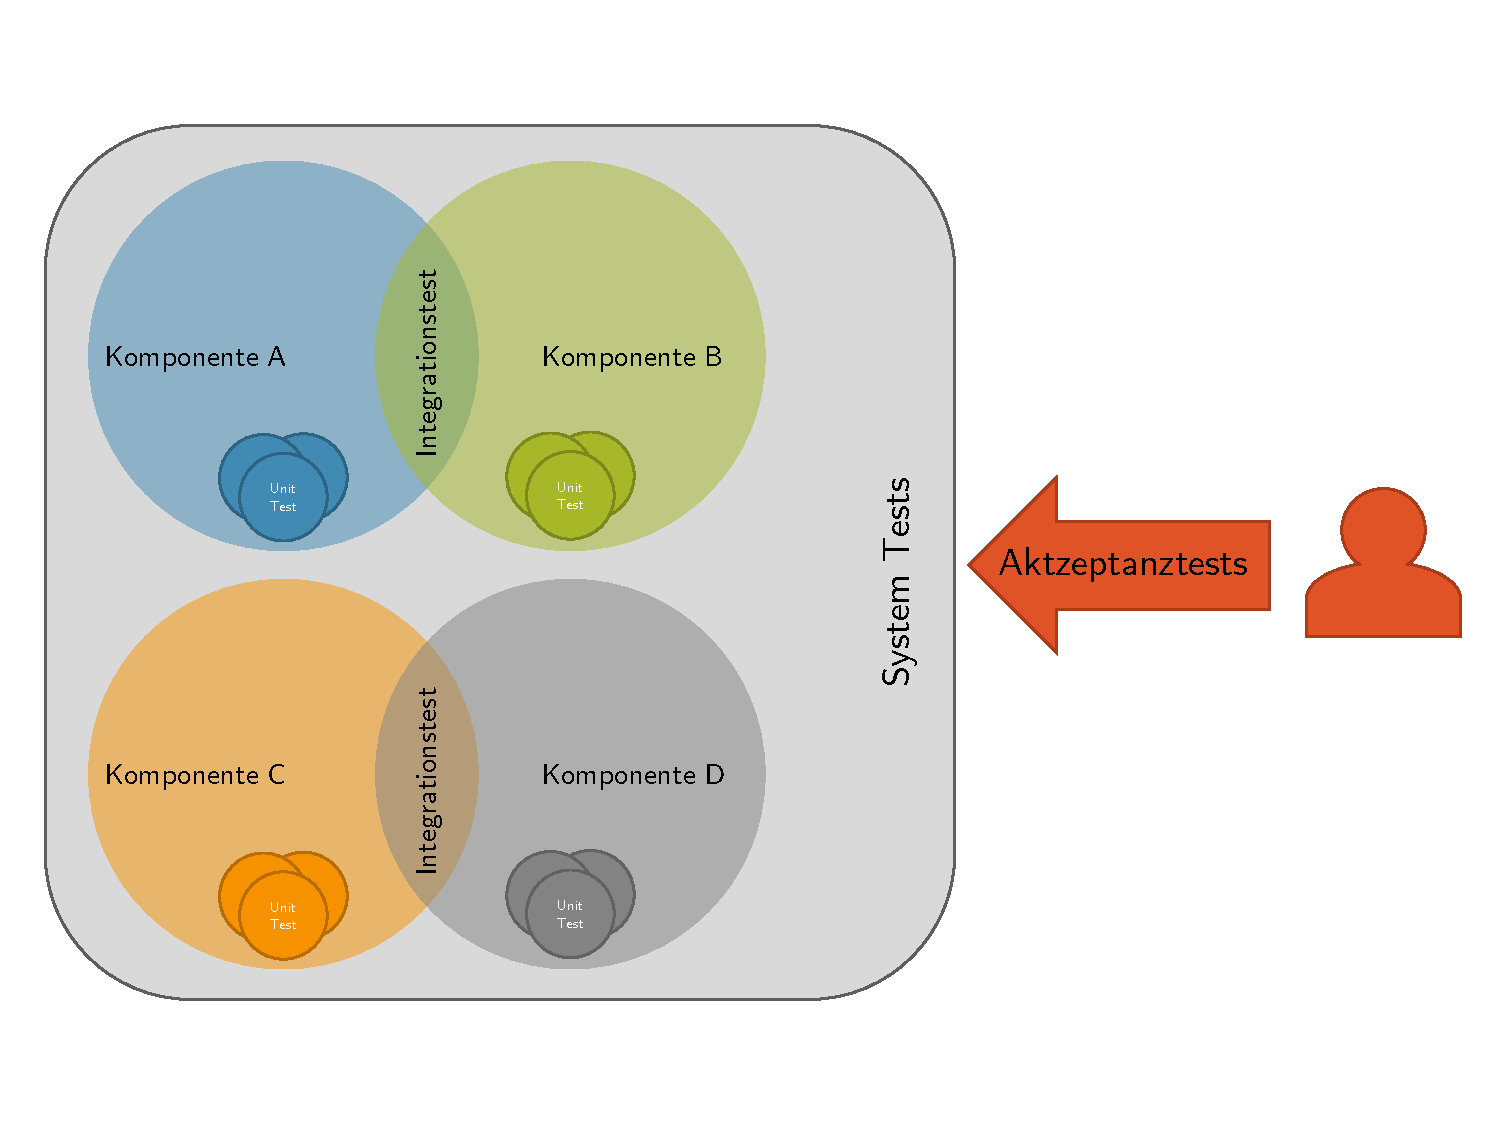
\includegraphics[width=0.9\linewidth]{images/img_testmethods_functional.pdf}
	\captionof{figure}[Bekannte Testmethoden]{Bekannte Testmethoden}
	\label{fig:img_testmethods_functional}
\end{minipage}
\end{comment}

\subsection{Testen von Microservices}\label{ch:ms-test}
\label{sec:testingms}

\paragraph{Unit Tests}


\begin{comment}
\vspace{1em}
\begin{minipage}{\linewidth}
	\centering
	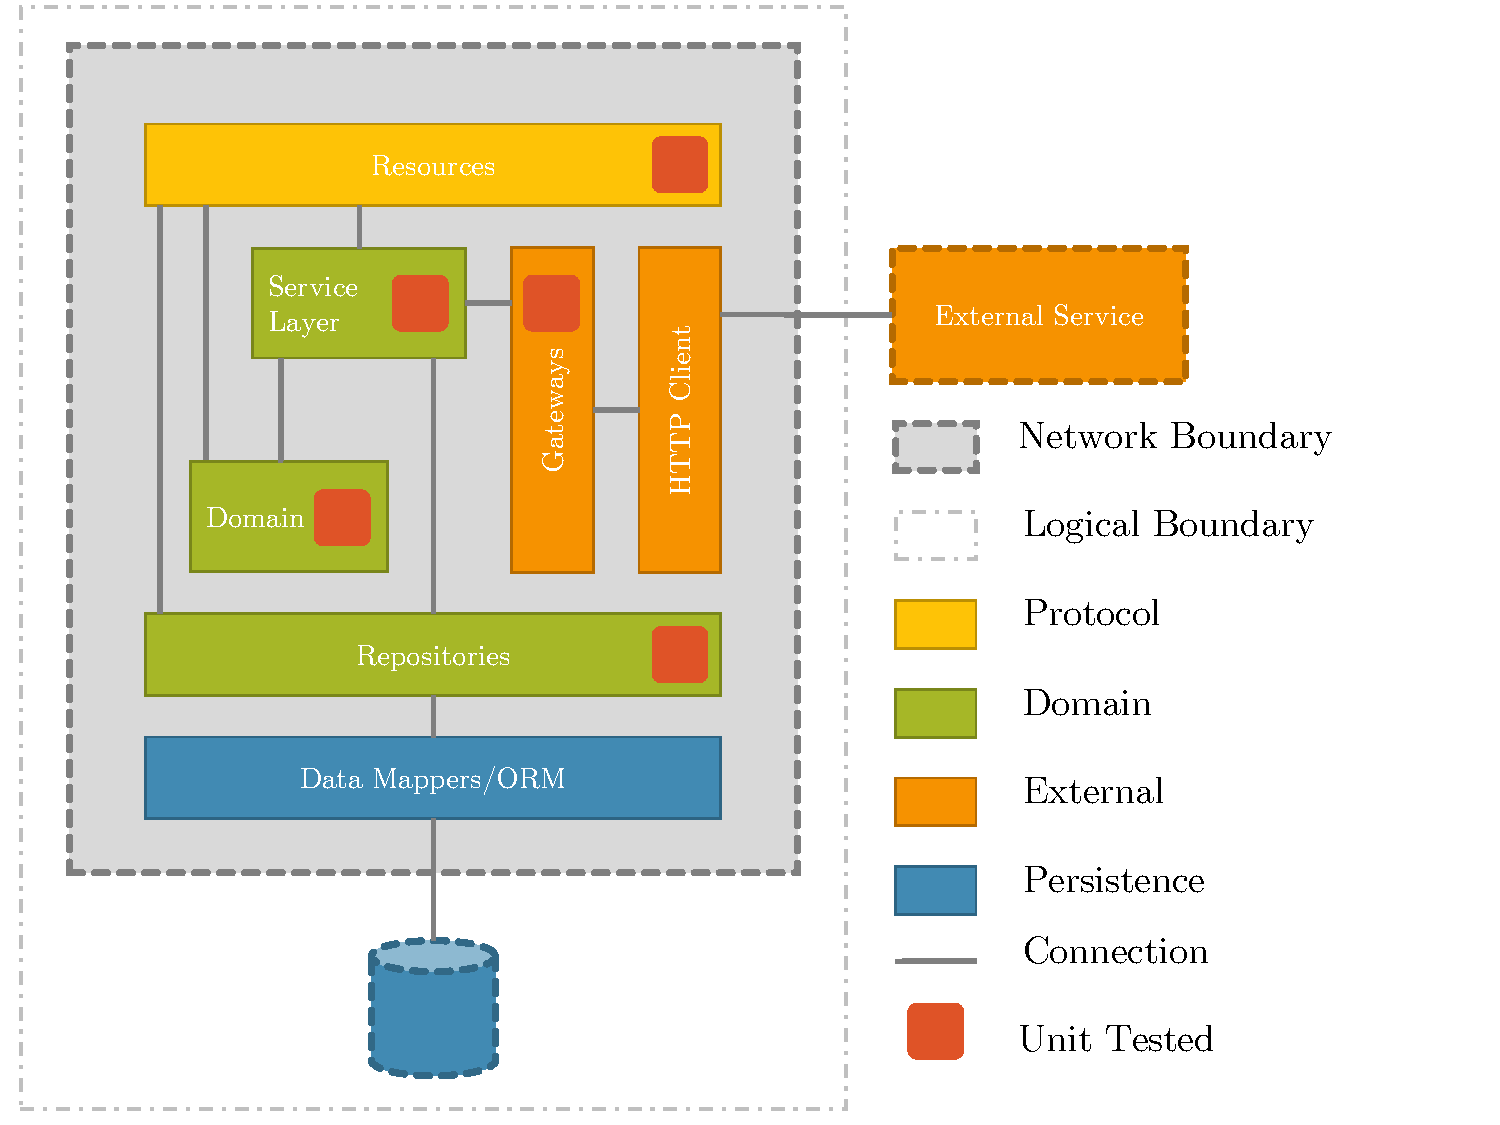
\includegraphics[width=0.9\linewidth]{images/img_unit-testing.pdf}
	\captionof{figure}[Unit Testing Scope]{Unit Testing Scope \cite{clemson}}
	\label{fig:img_unit-testing}
\end{minipage}
\end{comment}

\paragraph{Integrationstests}


\begin{comment}
\vspace{1em}
\begin{minipage}{\linewidth}
	\centering
	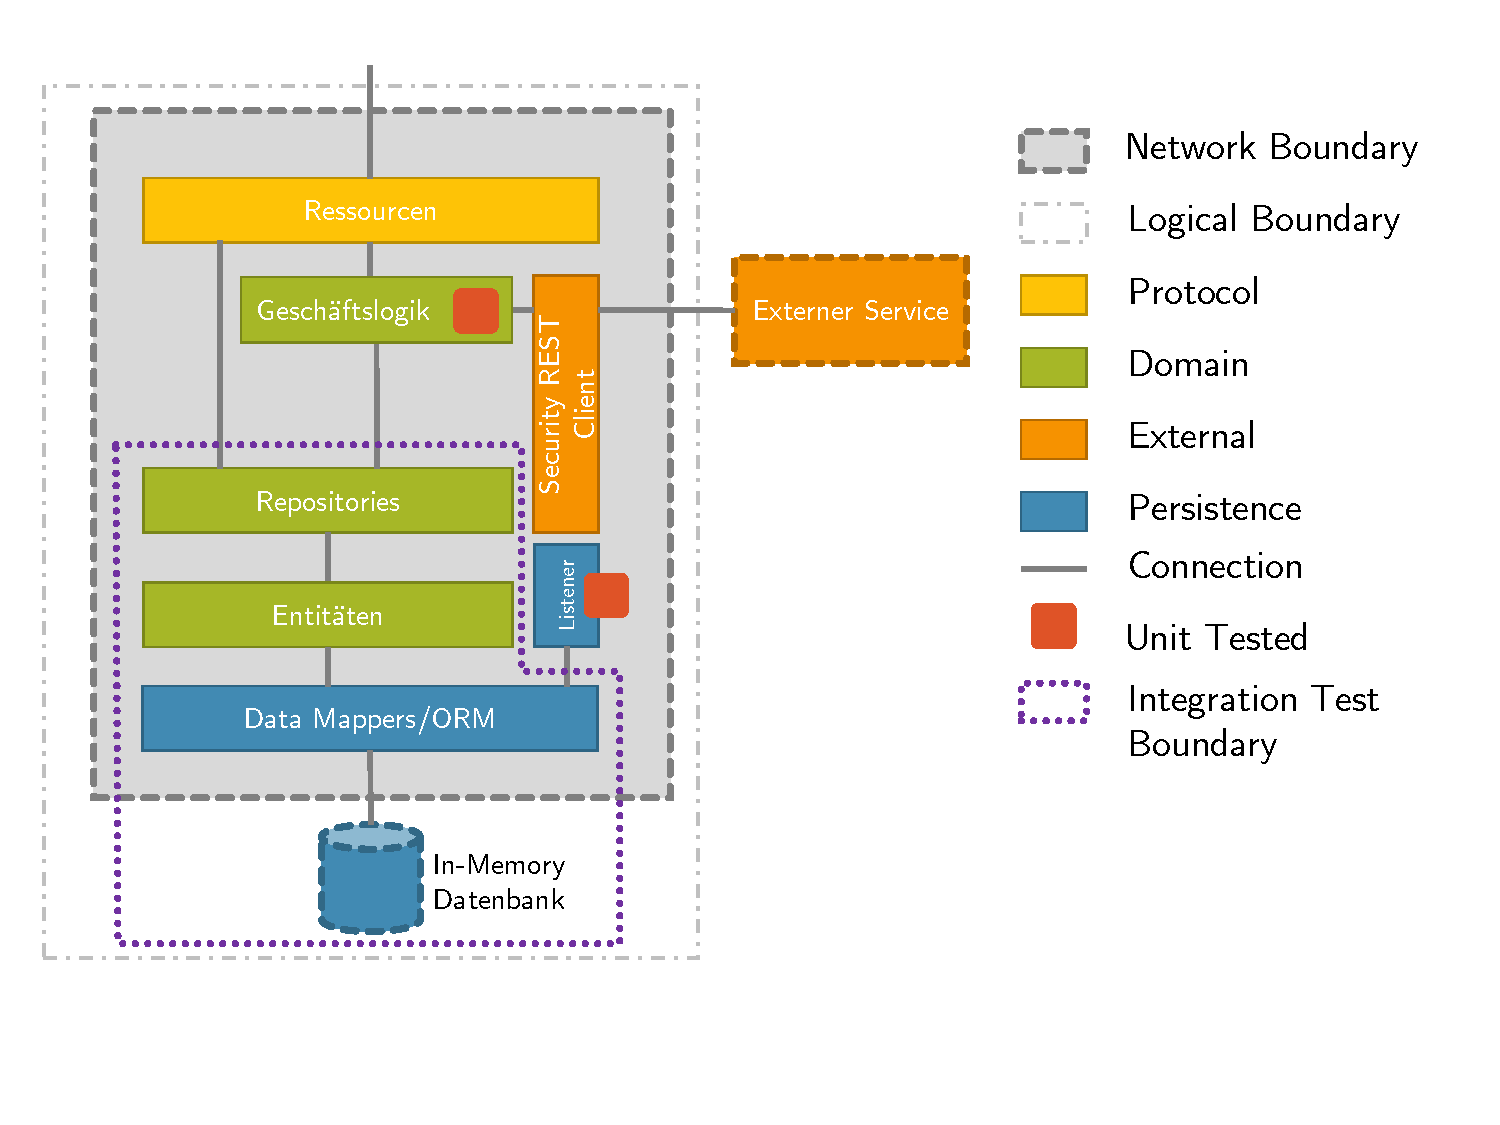
\includegraphics[width=0.9\linewidth]{images/img_integration-testing.pdf}
	\captionof{figure}[Integration Testing Scope]{Integration Testing Scope \cite{clemson}}
	\label{fig:img_integration-testing}
\end{minipage}
\end{comment}

\paragraph{Komponententests}

\begin{comment}
\vspace{1em}
\begin{minipage}{\linewidth}
	\centering
	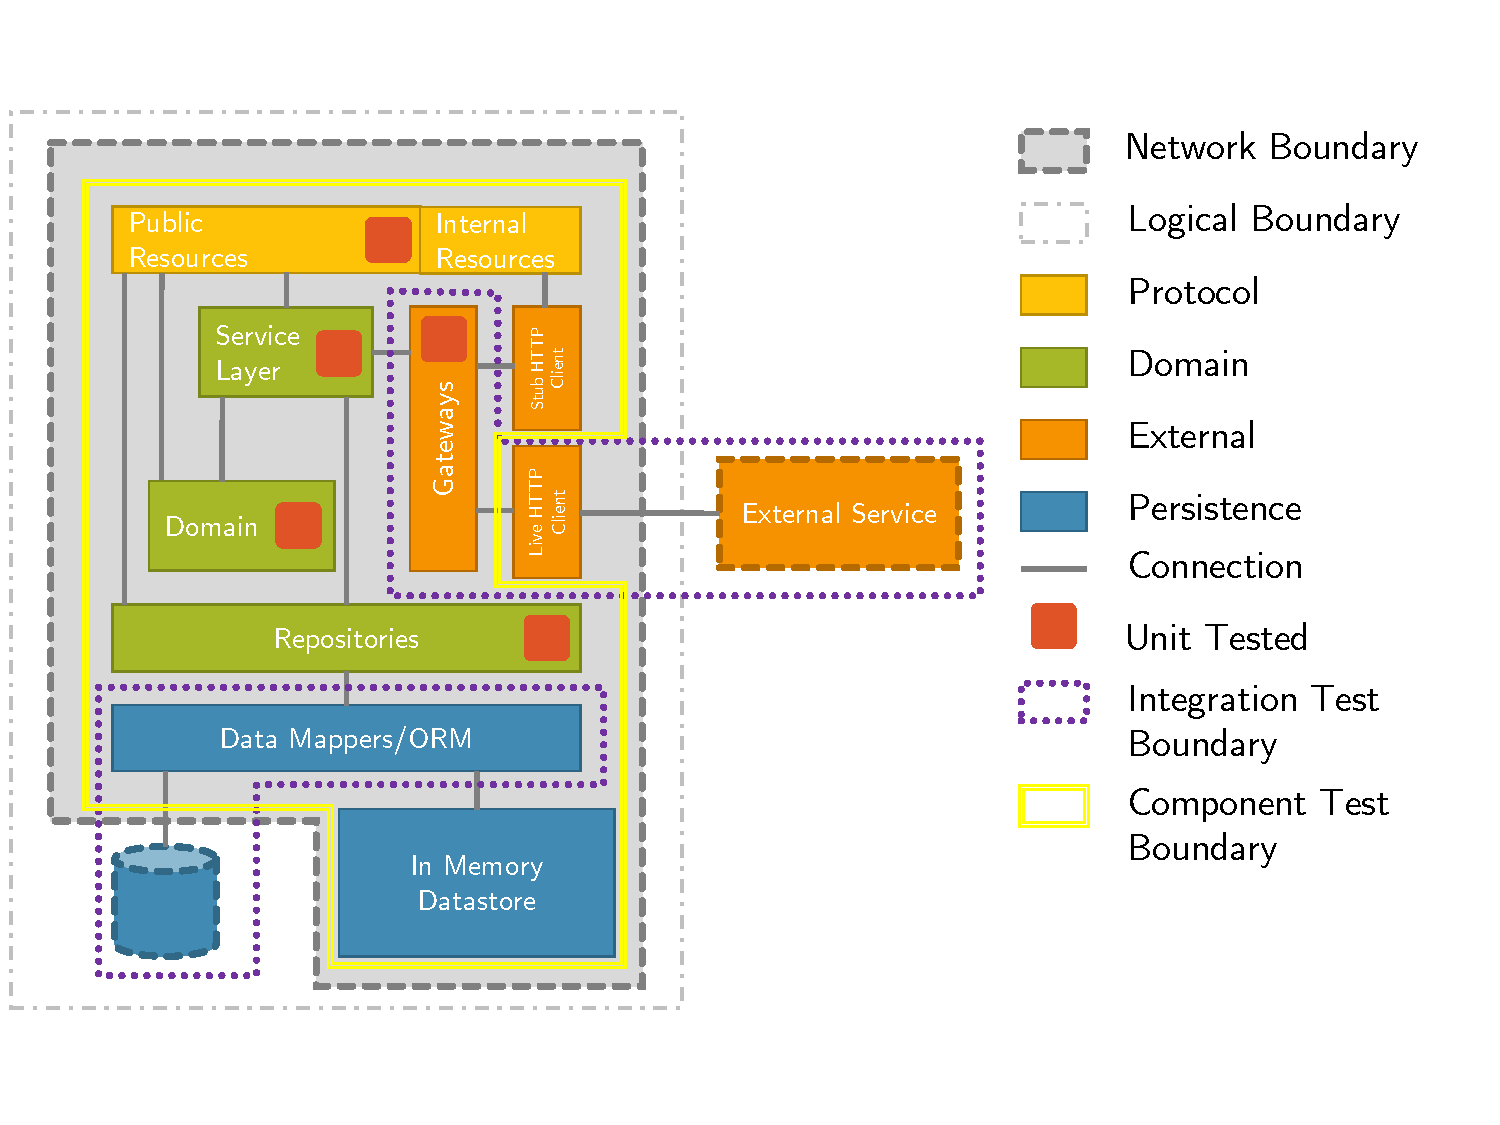
\includegraphics[width=0.9\linewidth]{images/img_component-testing.pdf}
	\captionof{figure}[Component Testing Scope]{Component Testing Scope \cite{clemson}}
	\label{fig:img_component-testing}
\end{minipage}
\end{comment}

\paragraph{Contract Testing}

\begin{comment}
\vspace{1em}
\begin{minipage}{\linewidth}
	\centering
	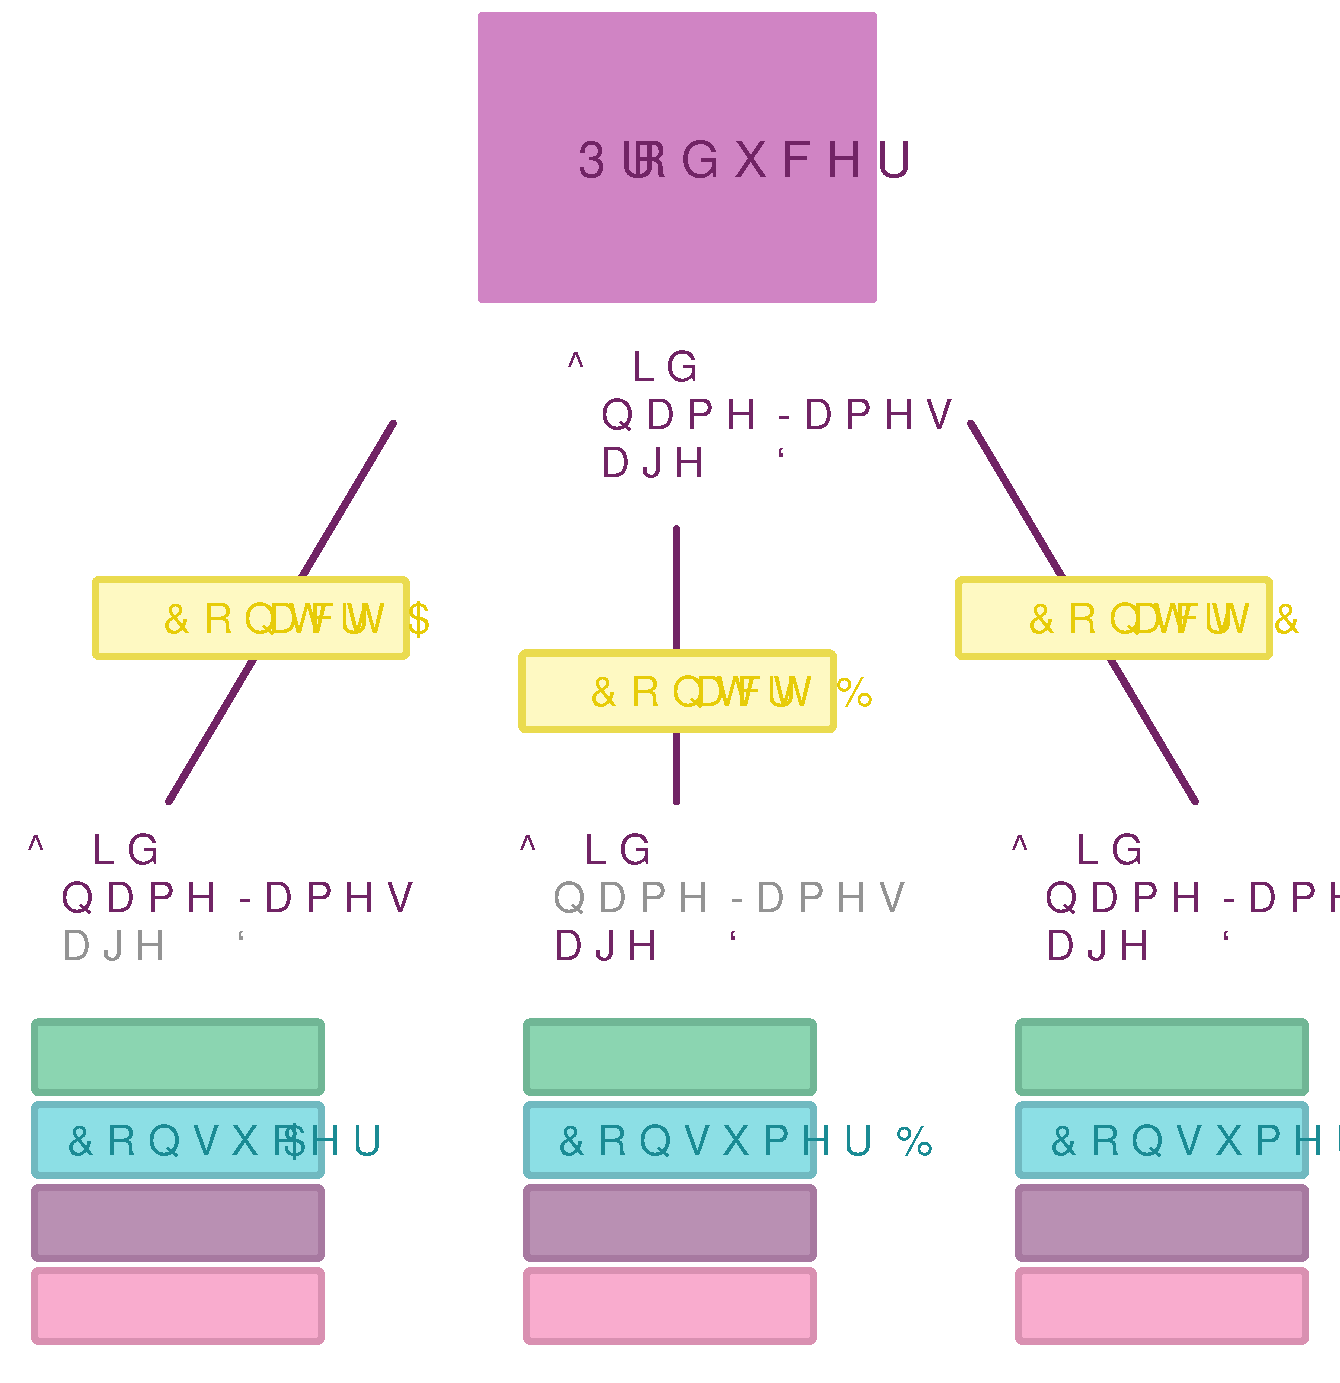
\includegraphics[width=0.9\linewidth]{images/img_contract-testing.pdf}
	\captionof{figure}[Contract Testing]{Contract Testing \cite{clemson}}
	\label{fig:img_contract-testing}
\end{minipage}
\end{comment}

\paragraph{End-To-End Testing}

\begin{comment}
\vspace{1em}
\begin{minipage}{\linewidth}
	\centering
	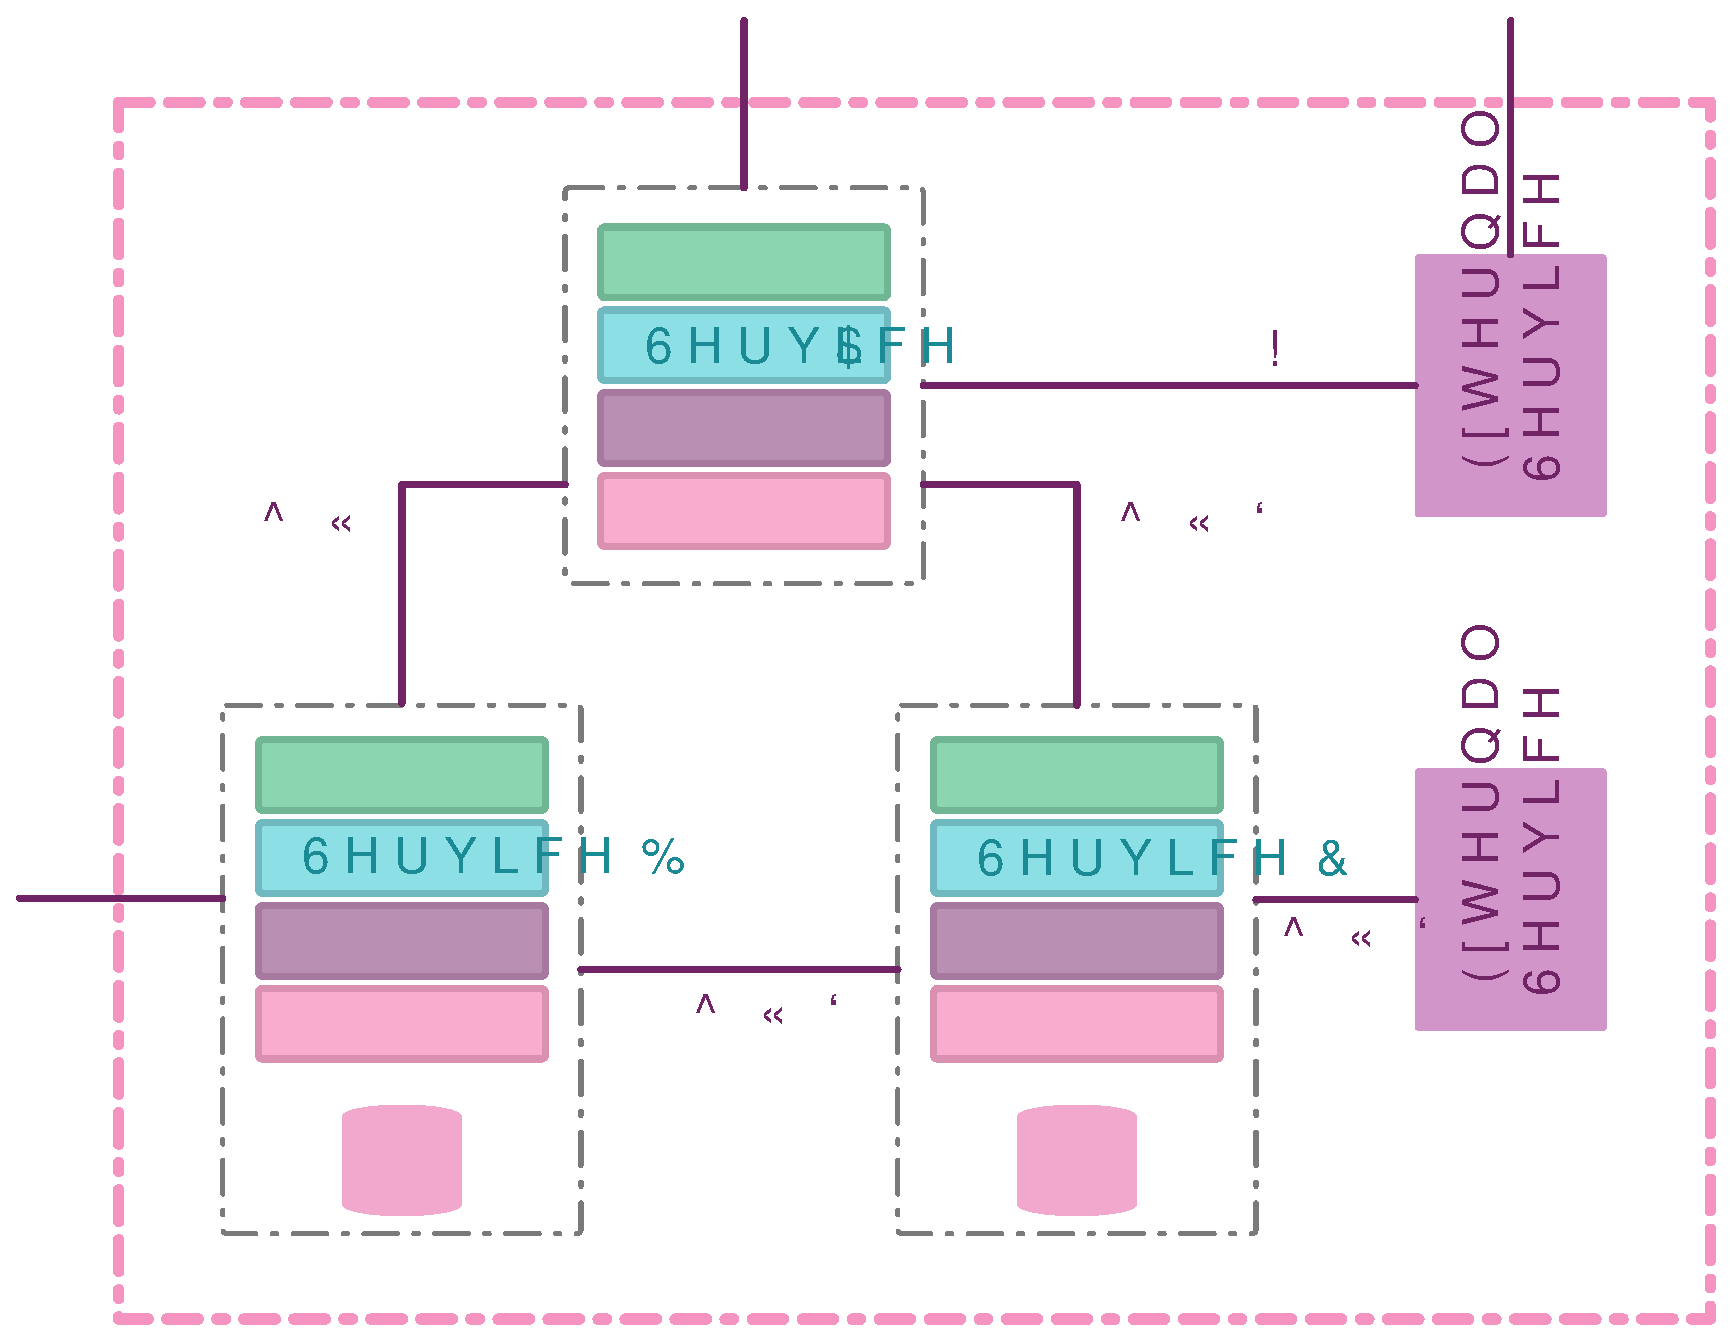
\includegraphics[width=0.9\linewidth]{images/img_end-to-end-testing.pdf}
	\captionof{figure}[End-To-End Testing Scope]{End-To-End Testing Scope \cite{clemson}}
	\label{fig:img_end-to-end-testing}
\end{minipage}
\end{comment}

\subsubsection{Sinnvolle Teststrategien für den generativen Ansatz}\label{ch:ms-gen-test}

\subsubsection{Frameworks zum Umsetzen von Test-Strategien}\label{ch:ms-test-frw}

% ----------------------------------------------------------------------------------------------------------
% Anforderungen an generierte Tests
% ----------------------------------------------------------------------------------------------------------
\section{Anforderungen an generierte Tests}\label{ch:anforderungen-tests}

\subsection{Benötigte Daten}

\subsection{Notwendige Änderungen/Erweiterungen von Barrakuda}

% ----------------------------------------------------------------------------------------------------------
% Implementierung in Barrakuda
% ----------------------------------------------------------------------------------------------------------
\section{Implementierung in Barrakuda}\label{ch:implementierung}

\subsection{Referenz-System}

Das Referenzsystem basiert auf der in Kapitel~\ref{ch:arch-itm} angesprochenen Architektur. Es wird das Spring-Framework verwendet. Auslöser dafür ist, dass bei it@M größtenteils Java-Entwickler arbeiten und diese bereits mit Java EE viel Erfahrung gesammelt haben. Da das Spring-Framework auf viele Konzepte von Java EE aufbaut, erleichtert dies den Einstieg in die Microservice-Welt für kommende Entwicklungen.

Die Services kommunizieren über eine REST-\ac{API}, die ihre Daten im JSON-Format überträgt. HATEOAS wird über Spring HATEOAS \footnote{\url{http://projects.spring.io/spring-hateoas/}} genutzt.

Als Datenbank in der Entwicklungsumgebung kommt eine In-Memory-Datenbank von H2 zum Einsatz. In der Produktion größtenteils Oracles JDBC-Datenbank in der Version 7, aber auch MySQL wird verwendet.

Zur Authentifizierung wird ein Authentifizierungs-Service genutzt, der zusätzlich zur internen Nutzer- und Rechteverwaltung auch eine Anbindung an das Stadtweite \ac{LDAP} bietet.

Das Problem der Findung von Service wird mithilfe von Netflixs Eureka-Service gelöst. Dieser bietet innerhalb einer Domäne einen Zentralen Anlaufpunkt für alle Services um sich dort zu vermerken, sowie Informationen über die Adressen von anderen Services einzuholen.

Clients können mit der Domäne über ein \ac{API}-Gateway kommunizieren (Netflix Zuul). Dieses öffnet nach außen eine einzige Schnittstelle, über die sowohl eine graphische Nutzeroberfläche aufgerufen, als auch die einzelnen Services kontaktiert werden können. Auch ermöglicht das Gateway den Zugriff auf bestimmte Endpunkte zur sperren, was für die Landeshauptstadt insbesondere für Software interessant ist, die sowohl interne, als auch externe Schnittstellen bieten soll.

Auch werden Docker-Konfigurationen verwendet, um die Continous Delivery mithilfe eines Container-Frameworks zu ermöglichen.

Es wird ein vereinfachtes Modell eines Online-Shops, beispielhaft \textit{Kongo} genannt, als Anwendungszweck herangezogen. Das Model in der Barrakuda-Sprache sieht folgendermaßen aus:

\lstinputlisting{../ReferenceSystem/.mdsd/referencesystem.barrakuda}

Das Referenz-System besteht aus 3 Services, dem \textit{shoppingcart}-Service, dem \textit{ordering}-Service und dem \textit{warehouse}-Service. Im \textit{warehouse} werden alle verfügbaren Produkte des Online-Shops verwaltet. Wenn ein Kunde nun eines der Produkte bestellen möchte, wird eine Anfrage an den \textins{shoppingcart}-Service gesendet, die die OID des Produktes, sowie die gewünschte Anzahl enthält.

Wenn ein Kunde dann eine Bestellung aufgeben möchte, geht eine Anfrage mit der OID des virtuellen Einkaufswagens an den \textit{ordering}-Service, der zusätzlich Schnittstellen zum erstellen einer Rechnung, sowie zum stornieren einer Bestellung bietet.

Der mit generierte Authentifizierungsservice dient als Kundenverwaltung.

%todo Klassendiagramm

Wichtig ist, dass im Referenz-System keinerlei Logik zu den modellierten Geschäftsanwendungen implementiert wird, sondern lediglich die im Abschnitt~\ref{sec:testingms} angesprochenen Testmethoden.

\subsubsection{Komponenten und Aufbau}

\subsubsection{Implementierung des Systems}

\subsubsection{Implementierung der Tests}

\subsection{Übernahme der Referenz-Implementierung in Barrakuda-Templates}

% ----------------------------------------------------------------------------------------------------------
% Fazit
% ----------------------------------------------------------------------------------------------------------
\section{Fazit}

% ----------------------------------------------------------------------------------------------------------
% Literatur
% ----------------------------------------------------------------------------------------------------------
\renewcommand\refname{Quellenverzeichnis}
\bibliographystyle{settings/bibstyle}
\bibliography{settings/bibfile}
\pagebreak

% ----------------------------------------------------------------------------------------------------------
% Anhang
% ----------------------------------------------------------------------------------------------------------
\pagenumbering{Roman}
\setcounter{page}{1}
\lhead{Anhang \thesection}

\begin{appendix}
\section*{Anhang}
\phantomsection
\addcontentsline{toc}{section}{Anhang}
\addtocontents{toc}{\vspace{-0.5em}}

\section{Code-Fragmente}
Viel Beispiel-Code

\end{appendix}

\end{document}
